\mode*
% Plataformas e instituciones:
% USA-MIT-Tedrake-TODDLER
% RABBIT-EMARO-Universidad de Nantes-
%\section[Justificaci\'on]{\iftagged{handout-tufte}{\textbf{\textcolor{blueun}{Justificaci\'on}}}{Justificaci\'on}}
\mode<article|presentation>{%
  \iftagged{handout-tufte}%
  {\vspace{-0.3cm}\section[Justificaci\'on]{\textbf{\textcolor{blueun}{Justificaci\'on}}}}%
  {\section[Justificaci\'on]{Justificaci\'on}}%
}%\mode<presentation>{\section[Justificaci\'on]{Justificaci\'on}}
\label{sec:justify}
\mode<presentation>{
  \begin{frame}[label=justificacion]
    \justificacionTime
    \frametitle{Por qu\'e esta investigaci\'on?}
    \begin{center}
      \LARGE \textbf{\textcolor{blueun}{Justificaci\'on}}
    \end{center}      
  \end{frame}
  \begin{frame}[label=laboratorios]
    \laboratoriosTime
    \frametitle{Por qu\'e esta investigaci\'on?}
    \framesubtitle{Universidades, Institutos, Centros y Laboratorios trabajando en Rob\'otica B\'ipeda}
    %\fbox{
      \parbox[c][0.9\textheight][c]{0.95\textwidth}{
        \only<1>{
          \begin{center}
            \textbf{\textcolor{blueun}{ALGUNAS UNIVERSIDADES}}
            
\includegraphics[width=0.95\textwidth]{../images/BipedInstitutesAndUniversities_0.png}
          \end{center}
        }
        \only<2>{
          \begin{center}
            \textbf{\textcolor{blueun}{ALGUNOS INSTITUTOS}}
            
\includegraphics[width=0.95\textwidth]{../images/BipedInstitutesAndUniversities_1.png}
          \end{center}
        }
      }
    %}
  \end{frame}
  \begin{frame}[label=plataformas]
    \plataformasTime
    \frametitle{Por qu\'e esta investigaci\'on?}
    \framesubtitle{Algunas plataformas b\'ipedas}
    %\fbox{
      \parbox[c][0.9\textheight][c]{0.95\textwidth}{
        \only<1>{
          \begin{center}
            \textbf{\textcolor{blueun}{Algunas plataformas en costos y tiempos}}
            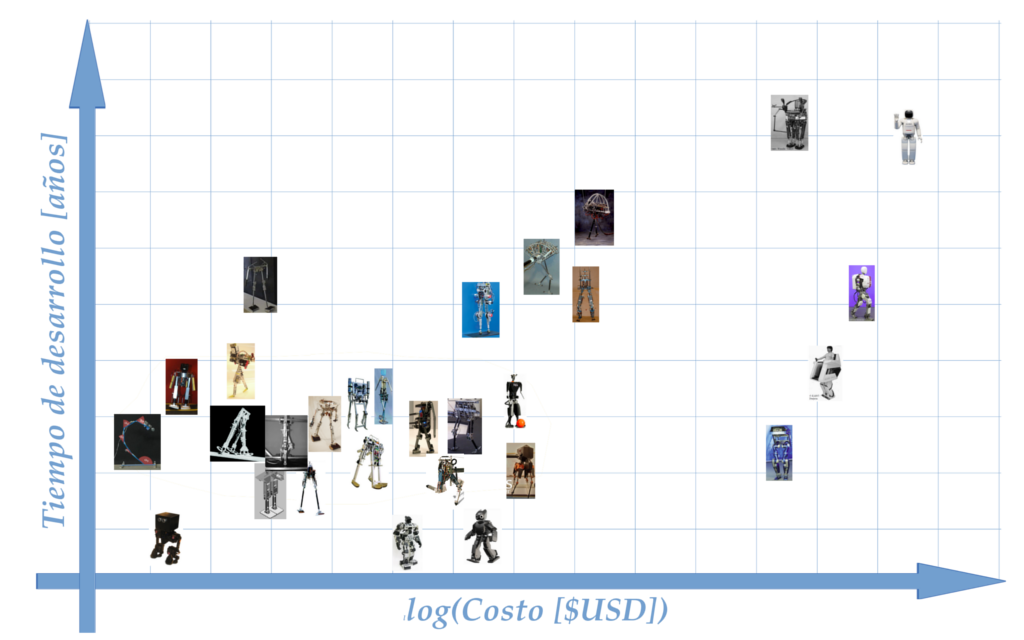
\includegraphics[width=0.95\textwidth]{../images/BipedPlatformsTime-Cost_small0.png}
          \end{center}
        }
        \only<2>{
          \begin{center}
            \textbf{\textcolor{blueun}{Bajos costos y tiempos de desarrollo}}
            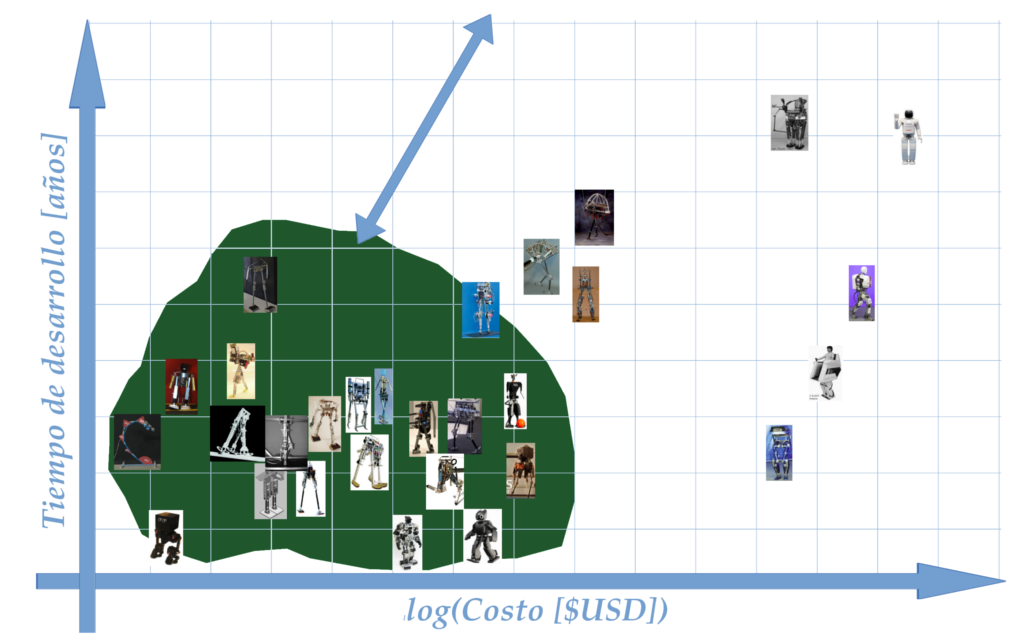
\includegraphics[width=0.95\textwidth]{../images/BipedPlatformsTime-Cost_small1.png}
          \end{center}
        }
        \only<3>{
          \begin{center}
            \textbf{\textcolor{blueun}{Trabajos de investigaci\'on en universidades}}
            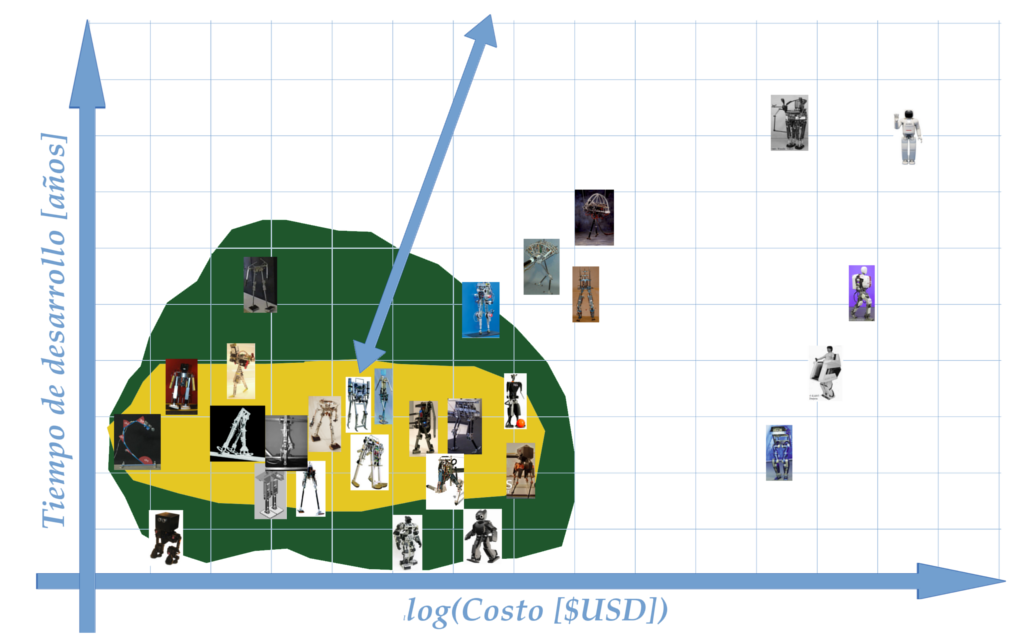
\includegraphics[width=0.95\textwidth]{../images/BipedPlatformsTime-Cost_small2.png}
          \end{center}
        }
      }
    %}
  \end{frame}
  \begin{frame}<1,2>[label=multidisciplinas]
    \multidisciplinasTime
    \frametitle{Por qu\'e esta investigaci\'on?}
    \framesubtitle{Trabajo multidisciplinario}
    \begin{center}
      \only<1-6,7>{
        \only<1-6>{\vspace{-2.0cm}}
        \only<7>{\vspace{-0.3cm}}
        \begin{columns}[c]
          \begin{column}{3cm}
            \only<1,3-7>{\setbeamercolor{postit}{fg=white,bg=red!50!black}}
            \only<2>{\setbeamercolor{postit}{fg=white,bg=red}}
            \hyperlink{exp_embebidos}{
              \begin{beamercolorbox}[sep=0.5em,wd=3cm,rounded=true,center,shadow=true]{postit}
                \only<1>{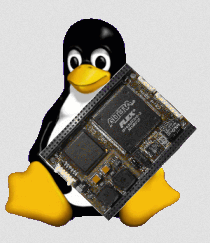
\includegraphics[height=1.5cm]{../images/ThemeEmbedded.png}\\}
                \only<2-6>{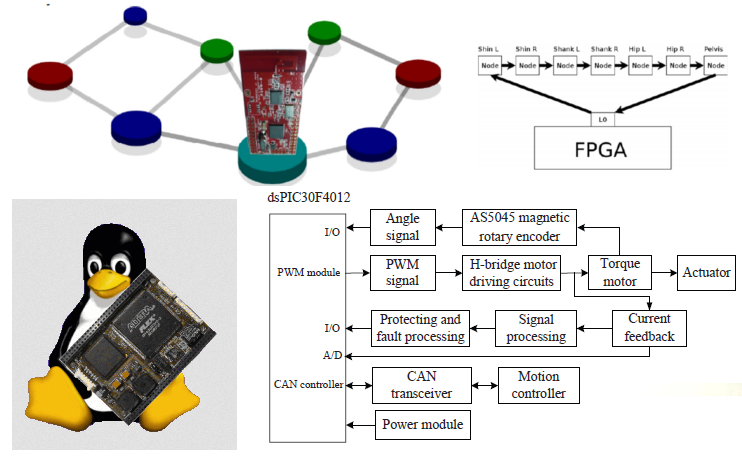
\includegraphics[height=1.5cm]{../images/ShortEmbedded.png}\\}
                \textbf{Sistemas Embebidos}
              \end{beamercolorbox}}
          \end{column}
          \begin{column}{3cm}
            \only<1-2,4-7>{\setbeamercolor{postit}{fg=white,bg=yellow!70!black}}
            \only<3>{\setbeamercolor{postit}{fg=white,bg=yellow}}
            \hyperlink{exp_biomecanica}{
              \begin{beamercolorbox}[sep=0.5em,wd=3cm,rounded=true,center,shadow=true]{postit}
                \only<1-2>{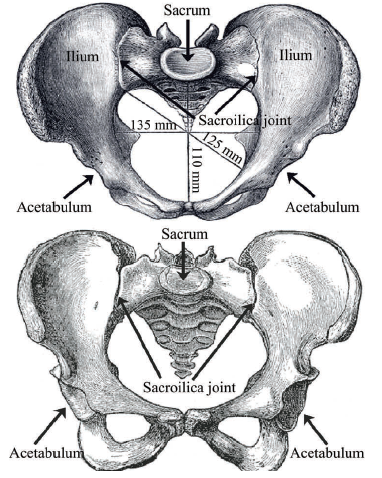
\includegraphics[height=1.5cm]{../images/ThemeBiomechanics.png}\\}
                \only<3-6>{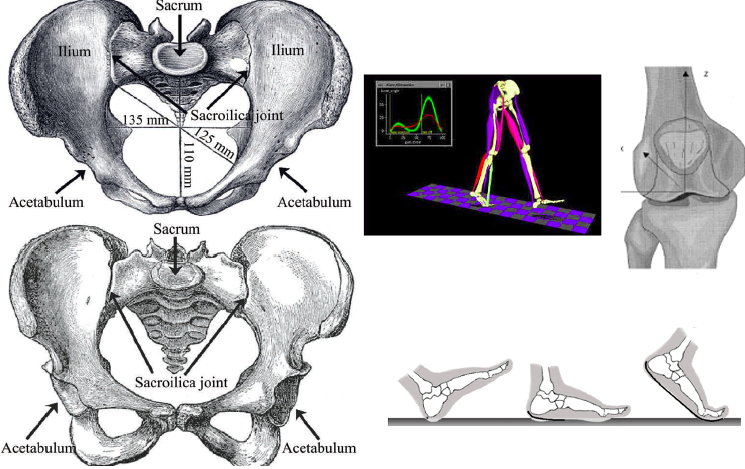
\includegraphics[height=1.5cm]{../images/ShortBiomechanics.png}\\}
                \textbf{Biomec\'anica}
              \end{beamercolorbox}}
          \end{column}
          \begin{column}{3cm}
            \only<1-3,5-7>{\setbeamercolor{postit}{fg=white,bg=blue!50!black}}
            \only<4>{\setbeamercolor{postit}{fg=white,bg=blue}}
            \hyperlink{exp_mecanismos}{
              \begin{beamercolorbox}[sep=0.5em,wd=3cm,rounded=true,center,shadow=true]{postit}
                \only<1-3>{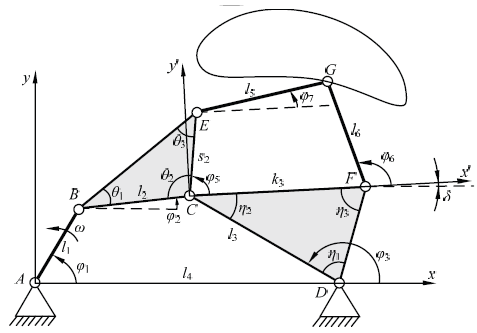
\includegraphics[height=1.5cm]{../images/ThemeMechanisms.png}\\}
                \only<4-6>{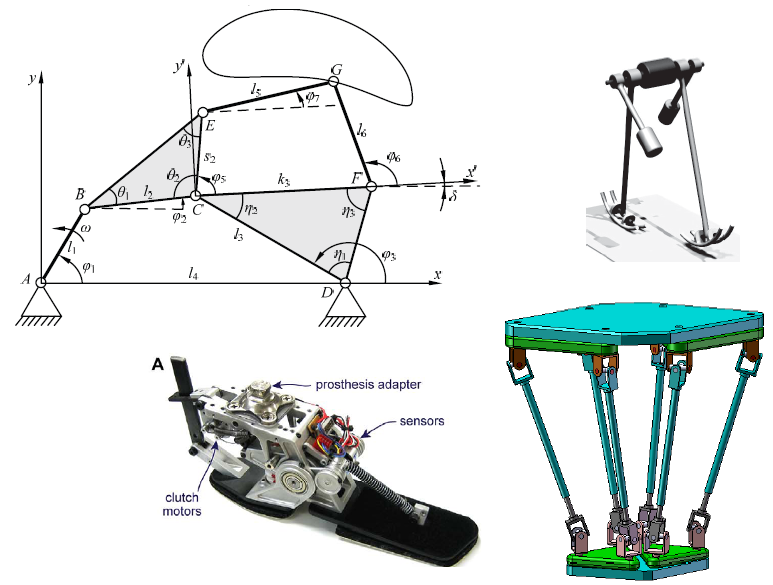
\includegraphics[height=1.5cm]{../images/ShortMechanisms.png}\\}
                \textbf{Modelado y Mecanismos}
              \end{beamercolorbox}}
          \end{column}
        \end{columns}
        \vspace{1.0cm}
        \begin{columns}[c]
          \begin{column}{3cm}
            \only<1-4,6-7>{\setbeamercolor{postit}{fg=white,bg=black}}
            \only<5>{\setbeamercolor{postit}{fg=white,bg=white!50!black}}
            \hyperlink{exp_computacion_flexible}{
              \begin{beamercolorbox}[sep=0.5em,wd=3cm,rounded=true,center,shadow=true]{postit}
                \textbf{C. Flexible y Optimizaci\'on}
                \only<1-4>{\\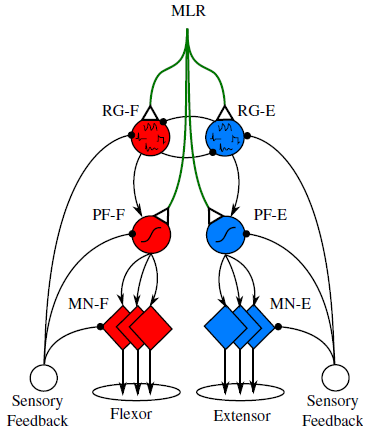
\includegraphics[height=1.5cm]{../images/ThemeSoftComputing.png}}
                \only<5-6>{\\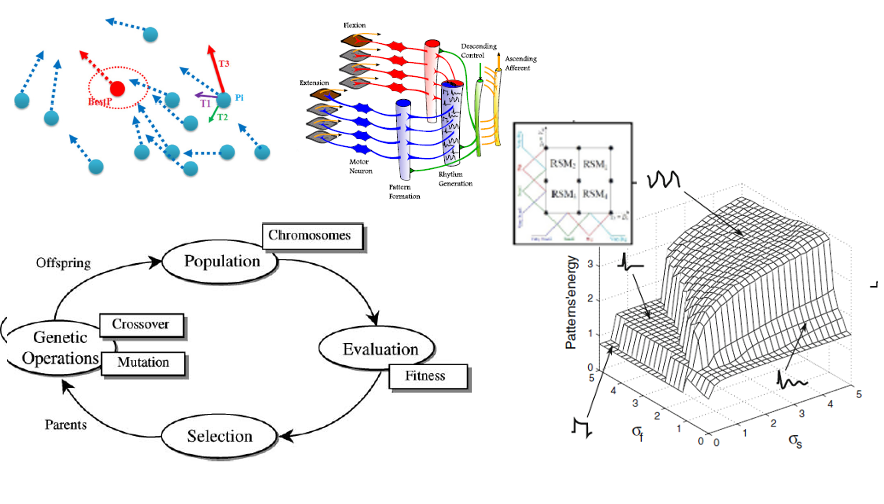
\includegraphics[height=1.5cm]{../images/ShortSoftComputing.png}}
              \end{beamercolorbox}}
          \end{column}
          \begin{column}{3cm}
            \only<1-5,7>{\setbeamercolor{postit}{fg=white,bg=green!50!black}}
            \only<6>{\setbeamercolor{postit}{fg=white,bg=green}}
            \hyperlink{exp_control}{
              \begin{beamercolorbox}[sep=0.5em,wd=3cm,rounded=true,center,shadow=true]{postit}
                \textbf{Control y Sis. Din\'amicos}
                \only<1-5>{\\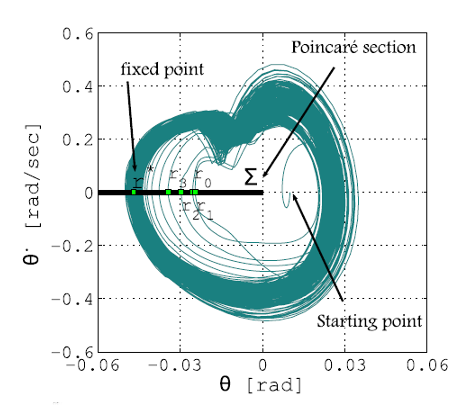
\includegraphics[height=1.5cm]{../images/ThemeControl.png}}
                \only<6-6>{\\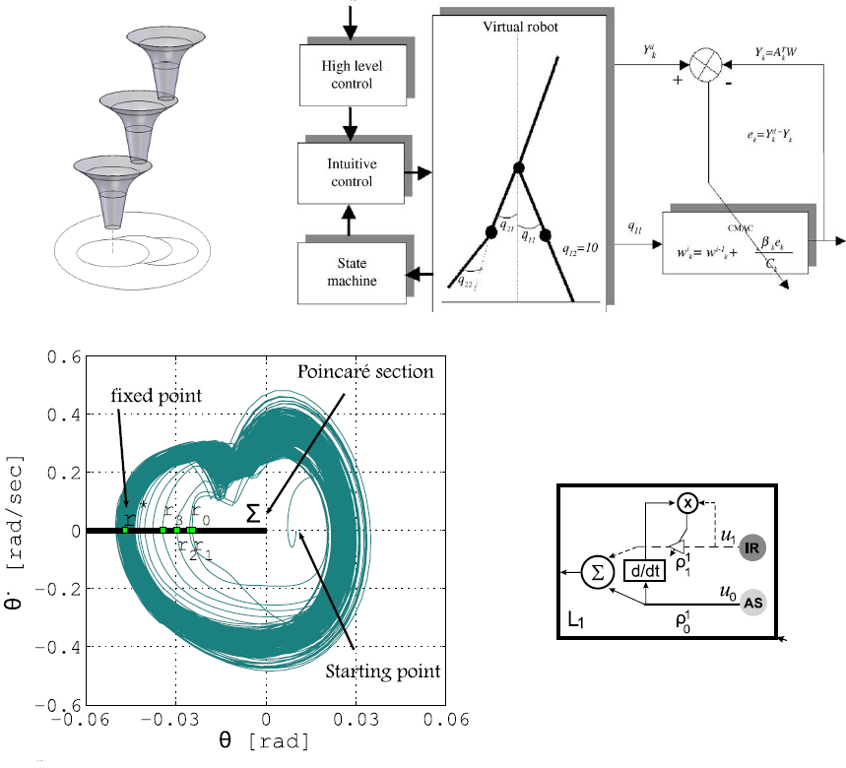
\includegraphics[height=1.45cm]{../images/ShortControl.png}}
              \end{beamercolorbox}}
          \end{column}
        \end{columns}
        \only<1-6>{\vspace{-4.6cm}}
        \only<7>{\vspace{-3.1cm}}
        \hspace{-0.1cm}
        \setbeamercolor{postit}{fg=white,bg=blueun}
        \begin{beamercolorbox}[sep=0.5em,wd=4.0cm,rounded=true,center]{postit}
          \textbf{\Large\textcolor{white}{ROB\'OTICA B\'IPEDA}}
        \end{beamercolorbox}
      }
    \end{center}
  \end{frame}
  % Explicaciones de diferentes ramas en convergencia a la rob\'otica b\'ipeda
  % SISTEMAS EMBEBIDOS
  \begin{frame}[plain,t,label=exp_embebidos]
    \expEmbebidosTime
    \hspace*{-0.8cm}\parbox[t]{\textwidth}{
      \only<1->{\vspace*{-0.4cm}\hspace*{-1.5cm}
        \colorbox{blueun}{
          \parbox[t][1.5cm][c]{\paperwidth}{
            \textcolor{white}{\Large\quad{SISTEMAS EMBEBIDOS}}
          }
        }
      }\vspace{0.05cm}\\\hspace*{-0.65cm}
      % \includegraphics[height=7.0cm]{../images/Embedded.png}}
      % 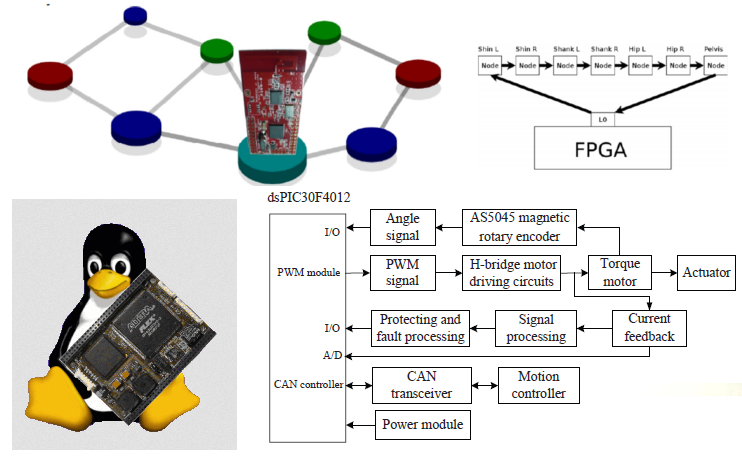
\includegraphics[height=7.0cm]{../images/ShortEmbedded.png}}
      % \animategraphics[height=7cm,autoresume,autoplay]{1}{../images/ShortEmbedded_}{0}{5}}
      \only<1>{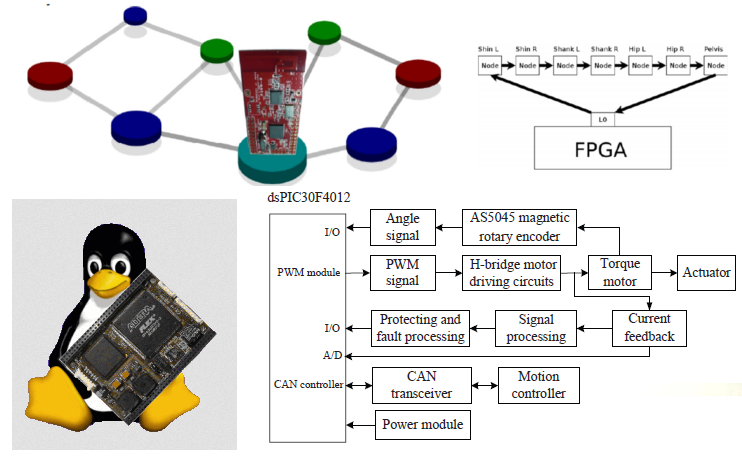
\includegraphics[height=7.0cm]{../images/ShortEmbedded_0.png}}%
      \only<2>{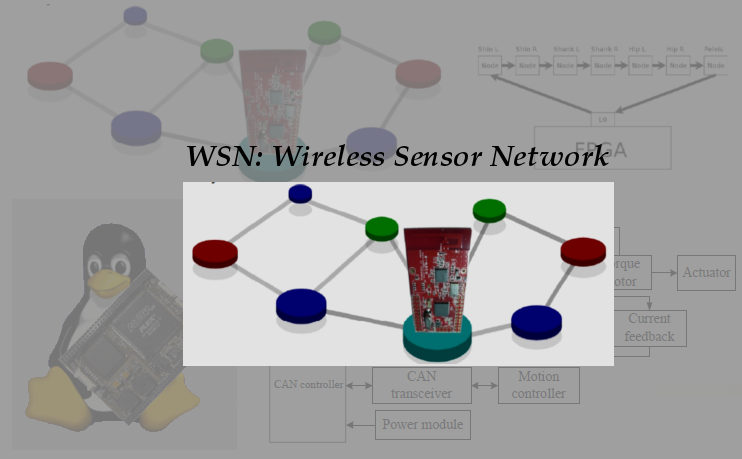
\includegraphics[height=7.0cm]{../images/ShortEmbedded_1.png}}%
      \only<3>{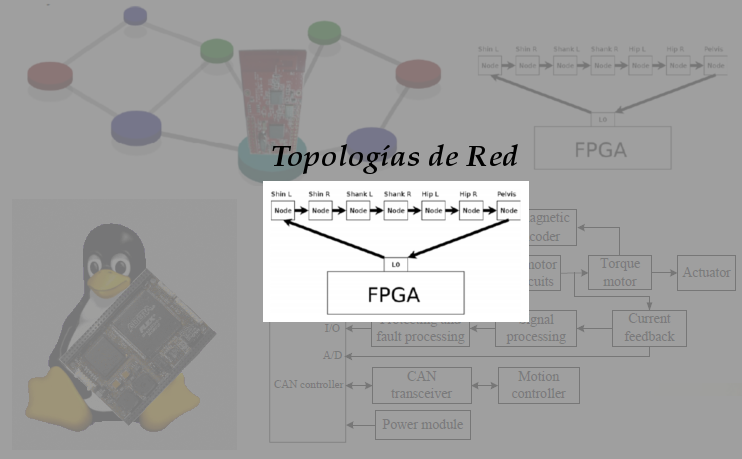
\includegraphics[height=7.0cm]{../images/ShortEmbedded_2.png}}%
      \only<4>{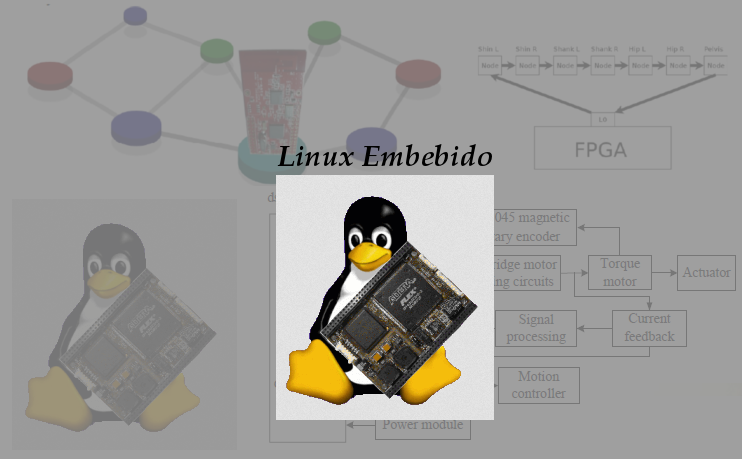
\includegraphics[height=7.0cm]{../images/ShortEmbedded_3.png}}%
      \only<5>{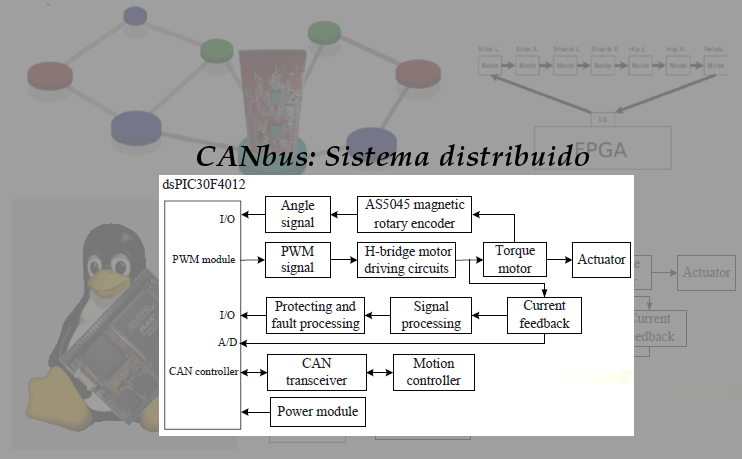
\includegraphics[height=7.0cm]{../images/ShortEmbedded_4.png}}%
      \only<6>{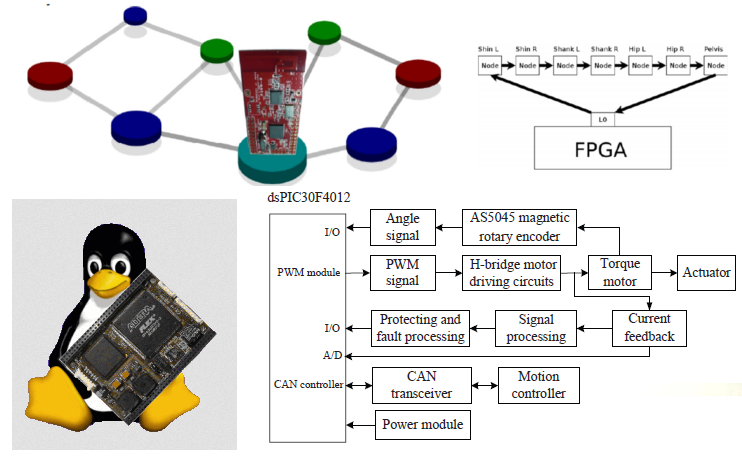
\includegraphics[height=7.0cm]{../images/ShortEmbedded_5.png}}%
    }
    \hyperlink<1->{multidisciplinas<2>}{\beamerreturnbutton{Volver}}
  \end{frame}
  \againframe<2-3>{multidisciplinas}
  % BIOMEC\'ANICA
  \begin{frame}[plain,t,label=exp_biomecanica]
    \expBiomecanicaTime
    \hspace*{-0.8cm}\parbox[t]{\textwidth}{
      \only<1-5>{\vspace*{-0.4cm}\hspace*{-1.5cm}
        \colorbox{blueun}{
          \parbox[t][1.5cm][c]{\paperwidth}{
            \textcolor{white}{\Large\quad{BIOMEC\'ANICA}}
          }
        }
      }\vspace{0.05cm}\\\hspace*{-0.5cm}
      % A\hspace{-1.5cm}\includegraphics[height=7.0cm]{../images/Biomechanics.png}}
      % A\hspace{-0.7cm}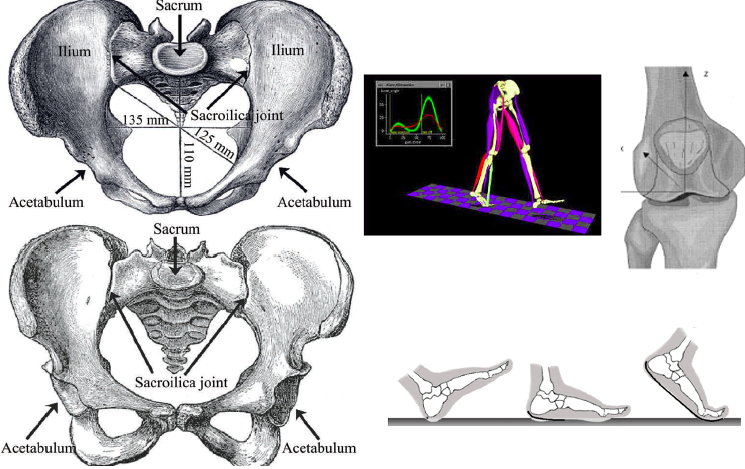
\includegraphics[height=7.0cm]{../images/ShortBiomechanics.png}}
      % \animategraphics[height=7cm,autoresume,autoplay]{0.8}{../images/ShortBiomechanics_}{0}{4}}
      \only<1>{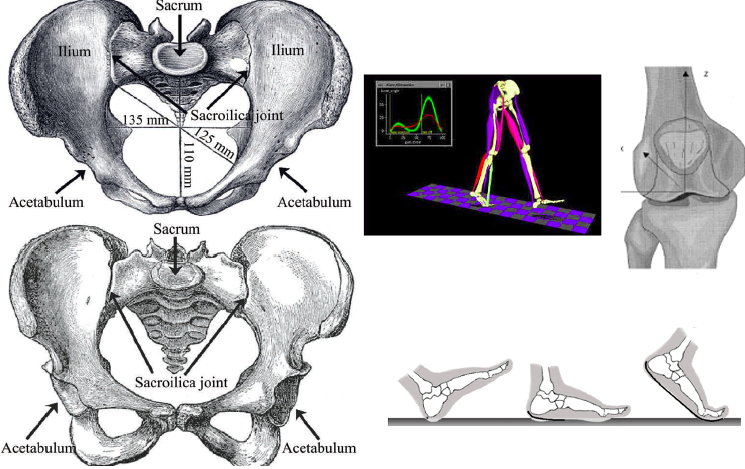
\includegraphics[height=7.0cm]{../images/ShortBiomechanics_0.png}}%
      \only<2>{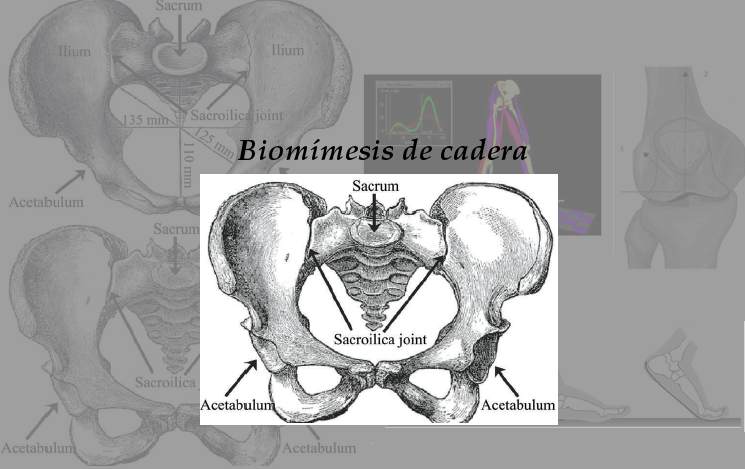
\includegraphics[height=7.0cm]{../images/ShortBiomechanics_1.png}}%
      \only<3>{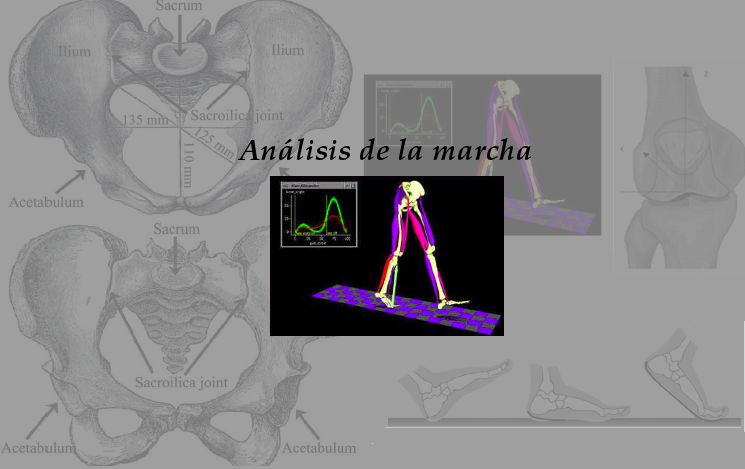
\includegraphics[height=7.0cm]{../images/ShortBiomechanics_2.png}}%
      \only<4>{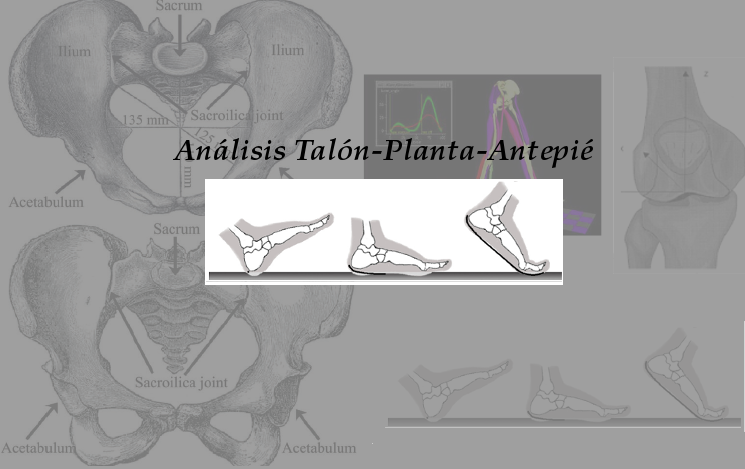
\includegraphics[height=7.0cm]{../images/ShortBiomechanics_3.png}}%
      \only<5>{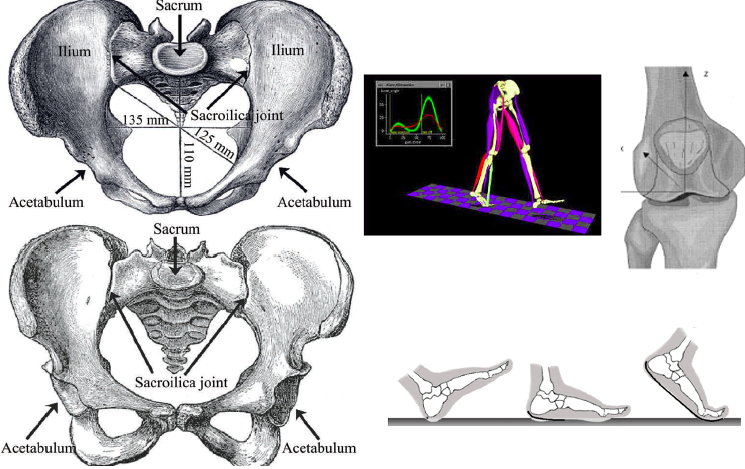
\includegraphics[height=7.0cm]{../images/ShortBiomechanics_4.png}}%
    }
    \hyperlink<1->{multidisciplinas<3>}{\beamerreturnbutton{Volver}}
  \end{frame}
  \againframe<3-4>{multidisciplinas}
  % MODELADO Y S\'ISNTESIS DE MECANISMOS
  \begin{frame}[plain,t,label=exp_mecanismos]
    \expMecanismosTime
    \hspace*{-0.8cm}\parbox[t]{\textwidth}{
      \only<1-6>{\vspace*{-0.4cm}\hspace*{-1.5cm}
        \colorbox{blueun}{
          \parbox[t][1.5cm][c]{\paperwidth}{
            \textcolor{white}{\Large\quad{Modelado de sistemas mec\'anicos y s\'intesis de mecanismos}}
          }
        }
      }\vspace{0.05cm}\\\hspace*{0.35cm}
      % \includegraphics[height=7.0cm]{../images/Mechanisms.png}}
      % 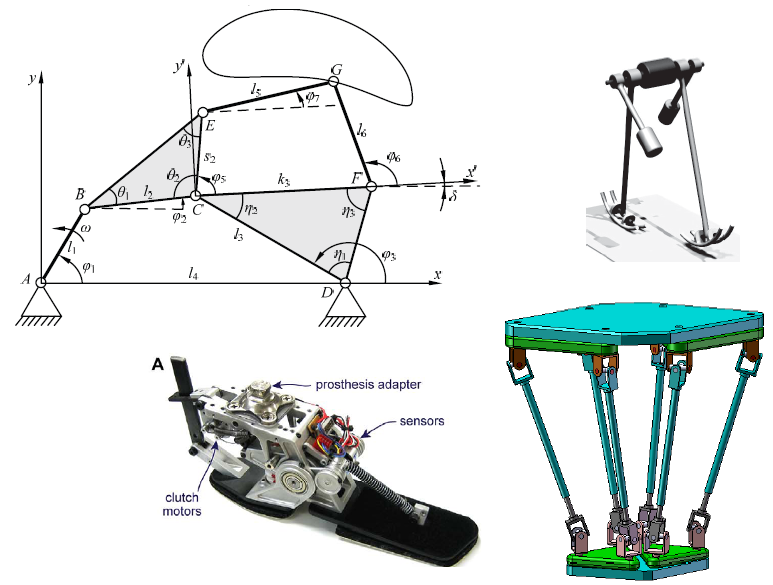
\includegraphics[height=7.0cm]{../images/ShortMechanisms.png}}
      % \animategraphics[height=7cm,autoresume,autoplay]{1}{../images/ShortMechanisms_}{0}{5}}
      \only<1>{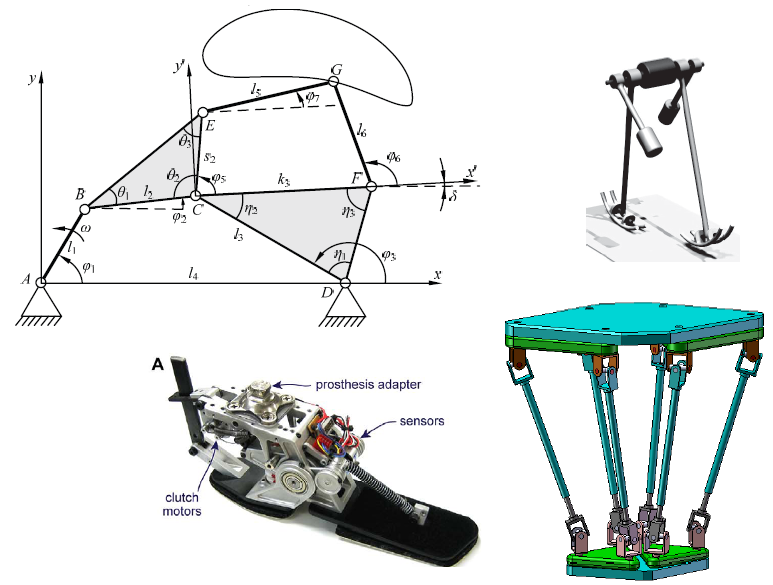
\includegraphics[height=7.0cm]{../images/ShortMechanisms_0.png}}%
      \only<2>{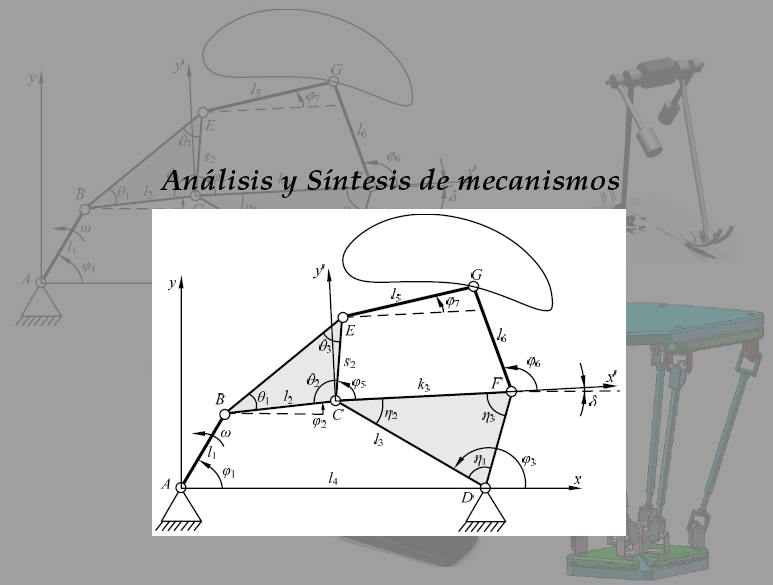
\includegraphics[height=7.0cm]{../images/ShortMechanisms_1.png}}%
      \only<3>{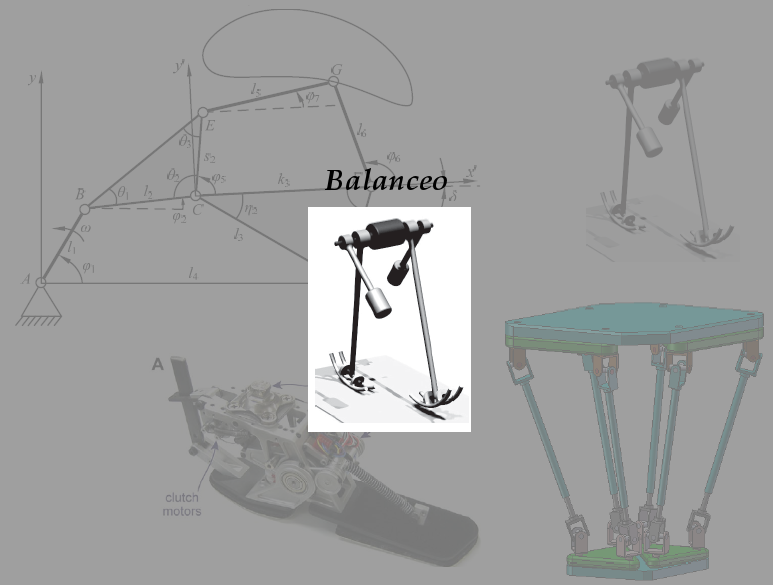
\includegraphics[height=7.0cm]{../images/ShortMechanisms_2.png}}%
      \only<4>{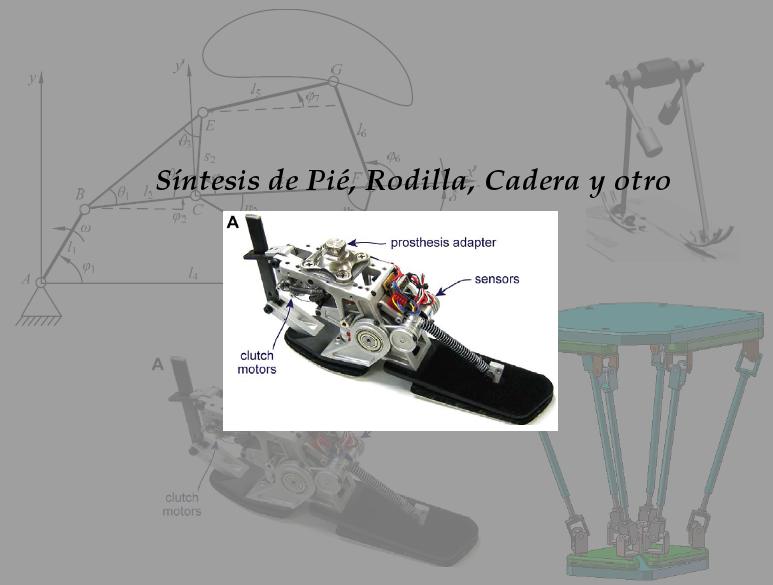
\includegraphics[height=7.0cm]{../images/ShortMechanisms_3.png}}%
      \only<5>{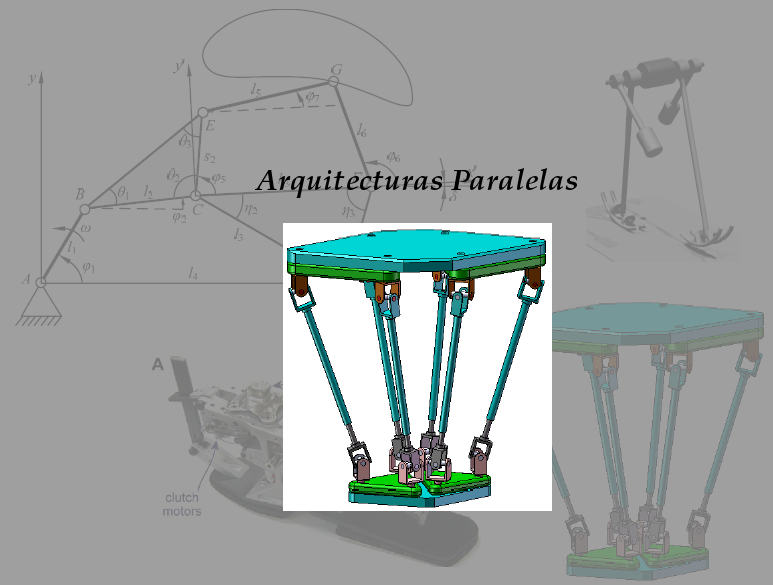
\includegraphics[height=7.0cm]{../images/ShortMechanisms_4.png}}%
      \only<6>{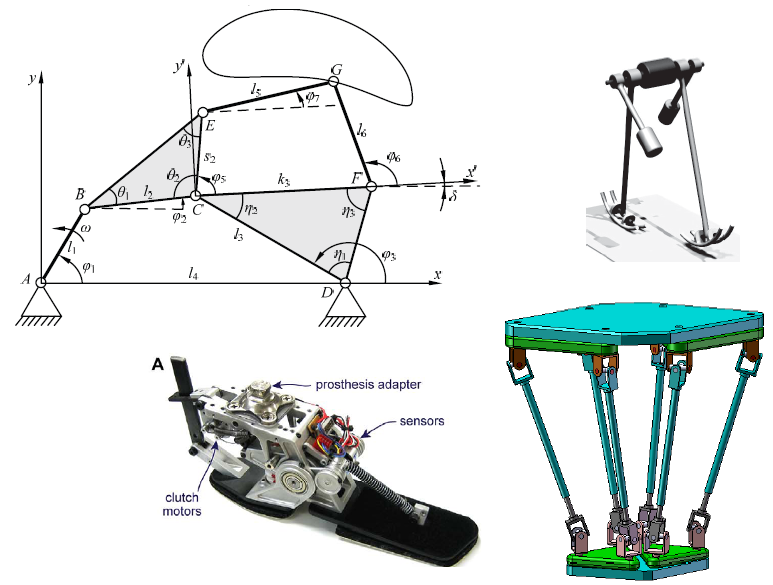
\includegraphics[height=7.0cm]{../images/ShortMechanisms_5.png}}%
    }
    \hyperlink<1->{multidisciplinas<4>}{\beamerreturnbutton{Volver}}
  \end{frame}
  \againframe<4-5>{multidisciplinas}
  % COMPUTACI\'ON FLEXIBLE
  % \only<5>{\textbf{\textcolor{blueun}{Optimizaci\'on, computaci\'on flexible e IA}}\\
  % \includegraphics[height=6.0cm]{../images/SoftComputing.png}}
  \begin{frame}[plain,t,label=exp_computacion_flexible]
    \expComputacionFlexibleTime
    \hspace*{-0.8cm}\parbox[t]{\textwidth}{
      \only<1-6>{\vspace*{-0.4cm}\hspace*{-1.5cm}
        \colorbox{blueun}{
          \parbox[t][1.5cm][c]{\paperwidth}{
            \textcolor{white}{\Large\quad{Optimizaci\'on, computaci\'on flexible e IA}}
          }
        }
      }\vspace{0.05cm}\\\hspace*{-1.1cm}
      % A\hspace{-1.0cm}\includegraphics[height=7.0cm]{../images/SoftComputing.png}}
      % A\hspace{-1.0cm}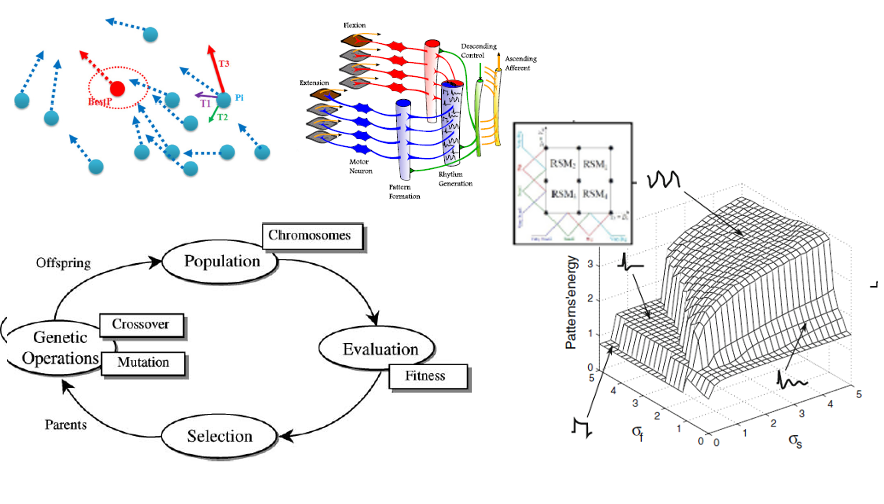
\includegraphics[height=7.0cm]{../images/ShortSoftComputing.png}}
      % \animategraphics[height=7cm,autoresume,autoplay]{1}{../images/ShortSoftComputing_}{0}{5}}
      \only<1>{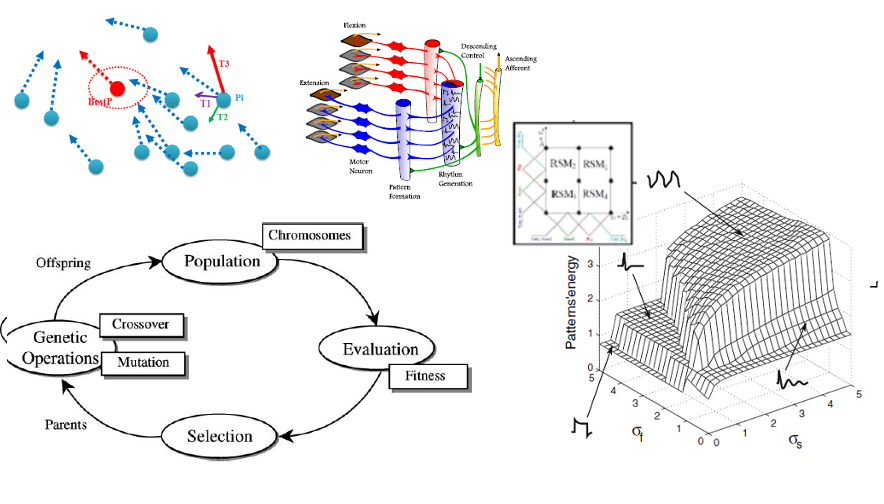
\includegraphics[height=7.0cm]{../images/ShortSoftComputing_0.png}}%
      \only<2>{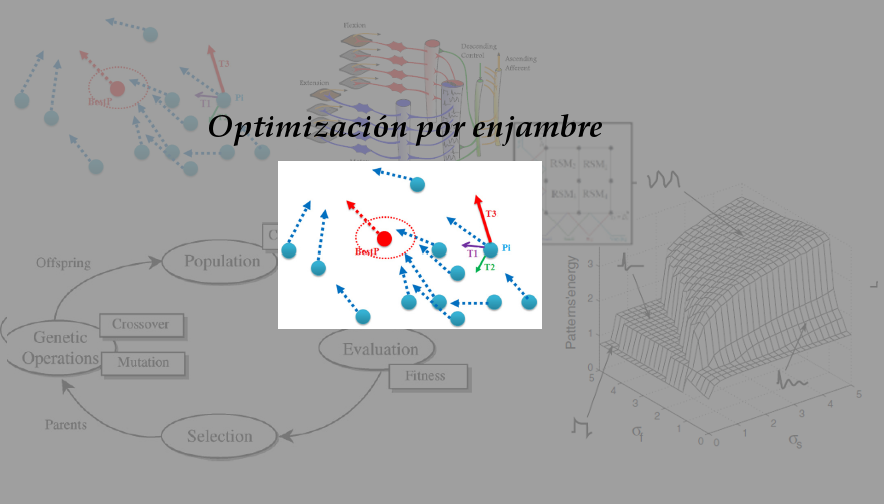
\includegraphics[height=7.0cm]{../images/ShortSoftComputing_1.png}}%
      \only<3>{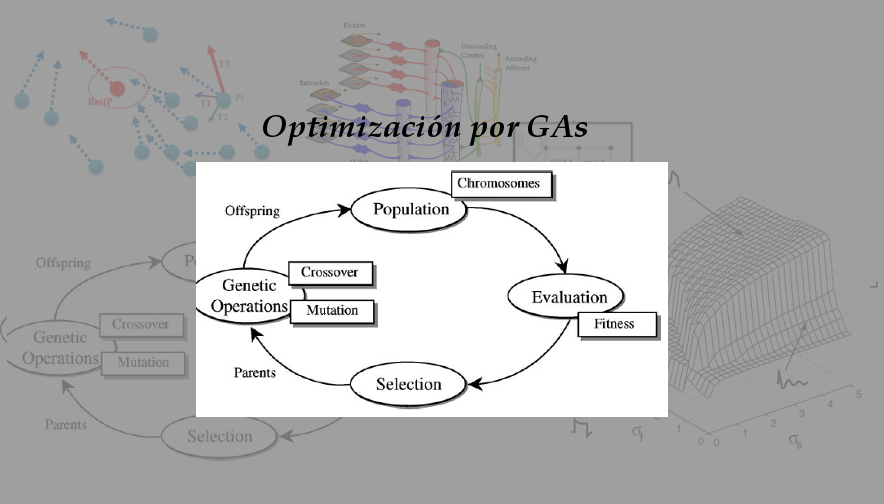
\includegraphics[height=7.0cm]{../images/ShortSoftComputing_2.png}}%
      \only<4>{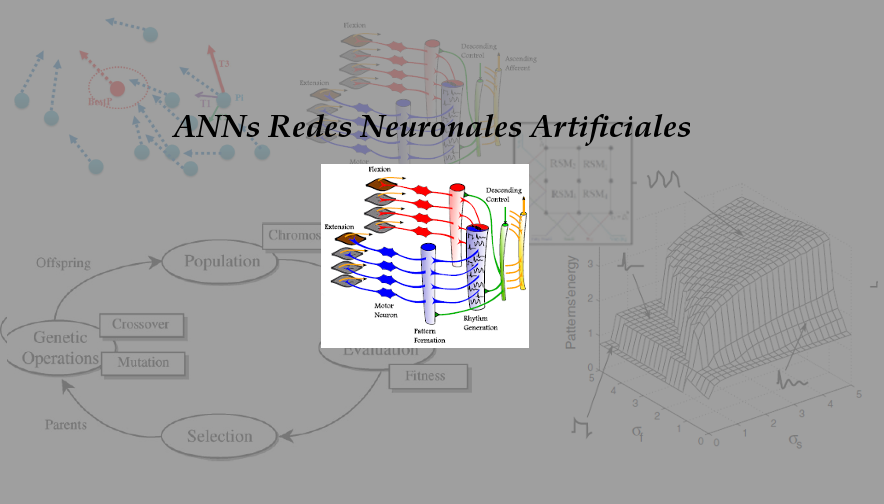
\includegraphics[height=7.0cm]{../images/ShortSoftComputing_3.png}}%
      \only<5>{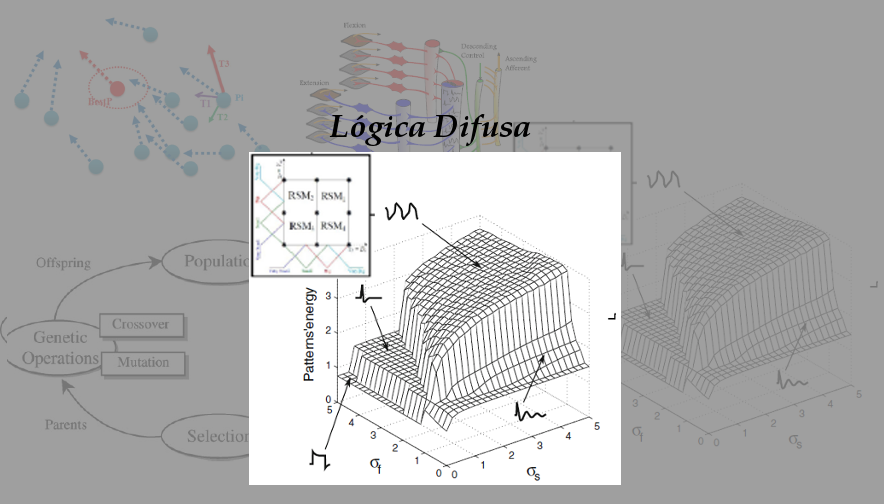
\includegraphics[height=7.0cm]{../images/ShortSoftComputing_4.png}}%
      \only<6>{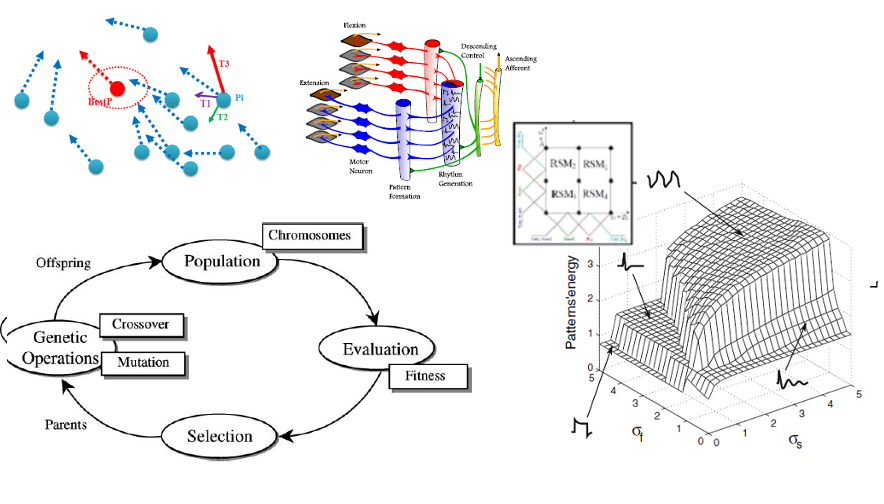
\includegraphics[height=7.0cm]{../images/ShortSoftComputing_5.png}}%
    }
    \hyperlink<1->{multidisciplinas<5>}{\beamerreturnbutton{Volver}}
  \end{frame}
  \againframe<5-6>{multidisciplinas}
  % CONTROL Y SISTEMAS DIN\'AMICOS
  % \only<6>{\textbf{\textcolor{blueun}{Control}}\\
  % \includegraphics[height=6.5cm]{../images/Control.png}}
  \begin{frame}[plain,t,label=exp_control]
    \expControlTime
    \hspace*{-0.8cm}\parbox[t]{\textwidth}{
      \only<1-6>{\vspace*{-0.4cm}\hspace*{-1.5cm}
        \colorbox{blueun}{
          \parbox[t][1.5cm][c]{\paperwidth}{
            \textcolor{white}{\Large\quad{Control y sistemas din\'amicos}}
          }
        }
      }\vspace{0.05cm}\\\hspace*{1.0cm}
      % \includegraphics[height=7.0cm]{../images/Control.png}}
      % \hspace{2.0cm}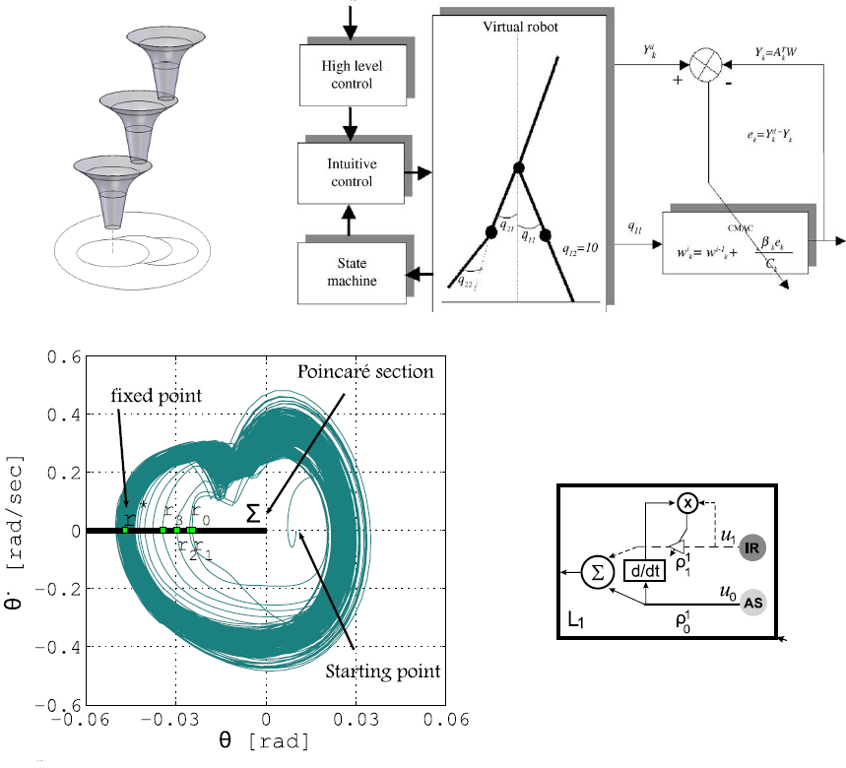
\includegraphics[height=7.0cm]{../images/ShortControl.png}}
      % \animategraphics[height=7cm,autoresume,autoplay]{1}{../images/ShortControl_}{0}{5}}
      \only<1>{\includegraphics[height=7.0cm]{../images/ShortControl_0.png}}%
      \only<2>{\includegraphics[height=7.0cm]{../images/ShortControl_1.png}}%
      \only<3>{\includegraphics[height=7.0cm]{../images/ShortControl_2.png}}%
      \only<4>{\includegraphics[height=7.0cm]{../images/ShortControl_3.png}}%
      \only<5>{\includegraphics[height=7.0cm]{../images/ShortControl_4.png}}%
      \only<6>{\includegraphics[height=7.0cm]{../images/ShortControl_5.png}}%
    }
    \hyperlink{multidisciplinas<6>}{\beamerreturnbutton{Volver}}
  \end{frame}
  \againframe<6->{multidisciplinas}
  % *********************************************************************************
  \subsection[Motivaci\'on]{Motivaci\'on}
  \label{sec:motiv}

  \begin{frame}[label=motivacion]
    \motivacionTime
    \frametitle{Por qu\'e esta investigaci\'on?}
    \framesubtitle{Algunos aspecto para la justificaci\'on}
    \quad\hspace{-0.8cm}\vspace{-0.5cm}
    \begin{columns}[T,totalwidth=0.97\textwidth]
      \small
      \begin{column}{0.55\textwidth}\setbeamercovered{transparent}
        \begin{enumerate}
        \item<1-|alert@1|uncover@1-6> Como ayuda de la proliferaci\'on
          \only<2-6>{
            \textit{\textbf{Ejemplo proceso de dise\~no:}}\setbeamercovered{transparent}
            \begin{itemize}\scriptsize
            \item<2-|alert@2|uncover@2> Bajo costo
            \item<3-|alert@3|uncover@3> Didacticos
            \item<4-|alert@4|uncover@4> Modularidad
            \item<5-|alert@5|uncover@5> Prototipado rapido
            \item<6-|alert@6|uncover@6> Metodologia de dise\~no
            \end{itemize}
          }
        \item<7-|alert@7|uncover@7-8> Motivaci\'on personal
        \item<9-|alert@9|uncover@9-19> Posibles productos y soluciones
          \only<9-19>{
            \begin{itemize}\scriptsize
            \setbeamercovered{transparent}
            \item<10-|alert@10|uncover@10-11> Teleoperaci\'on
            \item<12-|alert@12|uncover@12-13> Manufactura, transporte y ensambles
            \item<14-|alert@14|uncover@14-15> Movilidad en cuadrapl\'ejicos, pr\'otesis y caminata pasiva
            \item<16-|alert@16|uncover@16-17> Educaci\'on, cursos y materias
            \item<18-|alert@18|uncover@18-19> Entretenimiento e IA
            \end{itemize}
          }
        \item<20-|alert@20|uncover@20-32> Viabilidad
          \only<21-32>{
            \begin{itemize}\scriptsize\setbeamercovered{transparent}
            \item<21-|alert@21|uncover@21-22> Recursos f\'isicos
            \item<23-|alert@23|uncover@23-24> Profesores, grupos de investigaci\'on y materias
            \item<25-|alert@25|uncover@25-26> Convocatorias para recursos econ\'omicos y financiaci\'on
            \item<27-|alert@27|uncover@27-28> Relaciones con grupos internacionales de investigaci\'on
            \item<29-|alert@29|uncover@29-30> Experiencia del director de investigaci\'on en el tema
            \item<31-|alert@31|uncover@31-32> Experiencia del investigador en el tema del proyecto
            \end{itemize}
          }
        \item<33-|alert@33|uncover@33-38> Posible pasant\'ia
          \begin{itemize}\scriptsize
          \item<34-|alert@34|uncover@34> KUKA ROBOTICS
          \item<35-|alert@35|uncover@35> DLR-biped
          \item<36-|alert@36|uncover@36> Profesor M\'aximo Roa
          \item<37-|alert@37|uncover@37> Proyecto reciente
          \item<38-|alert@38|uncover@38> L\'ineas sugeridas de investigaci\'on
          \end{itemize}
        \end{enumerate}
      \end{column}
      \begin{column}{0.4\textwidth}
        \parbox[c][7cm][c]{4.0cm}{
          \only<1-4>{
            \begin{center}
              \includegraphics[height=7cm]{../images/RobotMR1_0.png}
            \end{center}
          }
          \only<5>{
            % \includegraphics[height=7cm]{../images/RobotMR1_0.png}
            \begin{center}
              \animategraphics[height=7cm,autoresume,autoplay]{3}{../images/RobotMR1_}{0}{12}
            \end{center}
          }
          \only<6>{
            \begin{center}
              \includegraphics[height=7cm]{../images/RobotMR1_12.png}
            \end{center}
            % \movie[width=3cm,height=7cm,externalviewer]{\includegraphics[height=7cm]{../images/RobotMR1_12.png}}{../videos/RobotMR1.flv} 
          }
          \only<8>{
            \begin{center}
              \animategraphics[height=7cm,autoresume,autoplay]{2}{../images/SomeThingsByMeSumary_}{0}{4}
              % \includegraphics[height=7.0cm]{../images/SomeThingsByMeSumary_0.png}
            \end{center}
          }
          \only<11>{
            \begin{center}
              \textbf{\textcolor{redun}{Teleoperaci\'on}}\\[0.3cm]
              \includegraphics[width=4.0cm]{../images/Teleoperacion.png}
            \end{center}
          }
          \only<13>{
            \begin{center}
              \textbf{\textcolor{redun}{Transporte}}\\[0.3cm]
              \includegraphics[width=4.0cm]{../images/Transporte.png}
            \end{center}
          }
          \only<15>{
            \begin{center}
              \textbf{\textcolor{redun}{Biomec\'anica}}\\[0.3cm]
              \includegraphics[width=4.0cm]{../images/ProsthesisAndPhysiotherapy.png}
            \end{center}
          }
          \only<17>{
            \begin{center}
              \textbf{\textcolor{redun}{Educaci\'on}}\\[0.3cm]
              \includegraphics[width=4.0cm]{../images/Educacion.png}
            \end{center}
          }
          \only<19>{
            \begin{center}
              \textbf{\textcolor{redun}{Entretenimiento}}\\[0.3cm]
              \includegraphics[width=4.0cm]{../images/Entretenimiento.png}
            \end{center}
          }
          \only<22>{
            \begin{center}
              \textbf{\textcolor{redun}{Recursos Disponibles}}
              \begin{itemize}\scriptsize
              \item CNC
              \item Impresoras 3D
              \item Software CAD-CAM-CAE
              \item Laboratorios con plataformas
              \end{itemize}
            \end{center}
          }
          \only<24>{
            \begin{center}
              \textbf{\textcolor{redun}{Lista de profesores}}
              \begin{enumerate}\tiny
              \item Din\'amica de robots\\{\tiny(R. Ram\'irez)}
              \item Biomec\'anica\\{\tiny(D. Garzon)}
              \item Sistemas embebidos\\{\tiny(C. Camargo)}
              \item Control de robots\\{\tiny(J. Sofrony)}
              \item Computaci\'on flexible\\{\tiny(V.H Grisales)}
              \item Aprendizaje de m\'aquina\\{\tiny(F. Gonz\'alez)}
              \item Optimizaci\'on\\{\tiny(A. Guzman)}
              \item Computaci\'on flexible\\{\tiny(L.F Ni\~no)}
              \item Inteligencia Artificial\\{\tiny(J. G\'omez)}
              \end{enumerate}
            \end{center}
          }
          \only<26>{
            \begin{center}
              \textbf{\textcolor{redun}{Convocatorias}}
              \begin{itemize}\scriptsize
              \item DIB
              \item VRi
              \item Colciencias
              \item Col-CAPES
              \item Col-DAAD
              \item Otras
              \end{itemize}
            \end{center}
          }
          \only<28>{
            \begin{center}
              \textbf{\textcolor{redun}{Posibles Relaciones}}
              \scriptsize
              \begin{itemize}
              \item Justin DLR (M. Roa)
              \item Robonaut 2 GM-NASA (L. Barajas)
              \item Walking Dynamics Conferences
              \item Clawar Conferences
              \end{itemize}
            \end{center}
          }
          \only<30>{
            \begin{center}
              \animategraphics[height=7cm,autoresume,autoplay]{1}{../images/SomeThingsByRR_}{0}{2}
              % \includegraphics[height=7.0cm]{../images/SomeThingsByRR_0.png}
            \end{center}
          }
          \only<32>{
            \scriptsize
            \begin{center}%P1(120,360),P2(1110,530)
              % \includegraphics[height=7cm]{../images/SomeThingsByMe_0.png}
              \animategraphics[height=7cm,autoresume,autoplay]{1.5}{../images/SomeThingsByMe_}{1}{5}
            \end{center}
          }
          \only<33-38>{
            \scriptsize
            \begin{center}%P1(120,360),P2(1110,530)
              \includegraphics[width=4cm]{../images/DLR-Roa-Tendencias.png}
            \end{center}
          }
        }
      \end{column}
    \end{columns}
    \only<28>{\vspace{-3.5cm}
      \begin{center}
        \includegraphics[width=0.95\textwidth]{../images/DynamicWalkingConferences.png}
      \end{center}
    }
  \end{frame}
}
\iftagged{handout-tufte}{%  
  \begin{marginfigure}[-7.0cm]%
    \centering
    \includegraphics{../images/BipedInstitutesAndUniversities_2.png}
    \caption{Universidades y laboratorios}
    \label{fig:uniAndLabs}
  \end{marginfigure}
  \vspace{-0.8cm}%
  \begin{figure}%[!htb]
    \centering
    \emph{\textcolor{blueun}{\textbf{Desarrollo en b\'ipedos con PhD Universitarios de poco tiempo}}}
    \includegraphics[width=8cm]{../images/BipedPlatformsTime-Cost_small2.png}    
    \caption{Desarrollo de plataformas en costo y tiempo}
    \label{fig:costoVsTiempo}
  \end{figure}%
  \begin{marginfigure}[-3.0cm]
    \centering
    % \includeslide[width=10cm]{multidisciplinas<6>}
    % \includegraphics{../images/Multidisciplinas.png}
    \includegraphics{../images/Multidisciplinas01.png}
    \caption{Multidisciplinas involucradas en la soluci\'on de problemas de la r\'obotica b\'ipeda}
    \label{fig:multi}
  \end{marginfigure}%
  \vspace{-0.3cm}%
  \begin{figure}
    \centering
    \includeslide[width=4.0cm]{exp_embebidos}
    \includeslide[width=4.0cm]{exp_biomecanica}\\
    \includeslide[width=4.0cm]{exp_mecanismos}\\
    \includeslide[width=4.0cm]{exp_computacion_flexible}
    \includeslide[width=4.0cm]{exp_control}
    \caption{Algunas figuras de los \'ultimos trabajos en rob\'otica b\'ipeda por \'area}
    \label{fig:multi_detalle}
  \end{figure}
}{Buscando una proliferaci\'on robusta de la rob\'otica en el pa\'is a nivel tecnol\'ogico y del conocimiento de esta \'area, se da acontinuaci\'on la justificaci\'on de este proyecto de investigaci\'on, propuesta que se ve acotada a ser trabajada en el mundo de la r\'obotica de caminadores.  Las tendencias a nivel mundial que se desarrollan en este tema actu\'almente, crecen cada d\'ia a pasos agigantados provocados por cientos de grupos de investigaci\'on pertenecientes a Universidades, Institutos, Centros y Laboratorios en todo el mundo.\par}
\untagged{handout-tufte}{Aunque la Universidad Nacional de Colombia ya comenz\'o sus investigaciones en el \'area con interesantes resultados\cite{M2005,M2005a,Roa2006,Heredia2007}, en donde se han construido lazos por medio de investigadores, profesores y estudiantes de la Universidad con otros grupos de vital importancia a nivel mundial en el \'area, como es el caso de \cite{Englsberger2011,Ott2011,M2013}. Desde hace unos siete a\~nos no se han desarrollado proyectos importantes en el \'area de caminadores.\par}
\untagged{handout-tufte}{El campo de la rob\'otica b\'ipeda ha superado\untagged{handout-tufte}{ algunos} problemas \untagged{handout-tufte}{y han surgido unos nuevos, en donde las soluciones encontradas han sido generadas} integrando m\'ultiples fuentes de conocimiento, en \'areas como: los sistemas embebidos\iftagged{handout-tufte}{}{\cite{Barker2010,Pan2010,Kimm2012,Wang2011,Amir2013}}, la biomec\'anica\iftagged{handout-tufte}{}{\cite{Mahmoodi2013,Lim2014,Wu2013,Aoustin2013,Chiang2013,Xiang2010,Hobon2014}}, el modelado de sistemas mec\'anicos\iftagged{handout-tufte}{}{\cite{Chiang2013}}, la s\'intesis de mecanismos\iftagged{handout-tufte}{}{\cite{Li2008,Aoustin2013,Wu2013a,Xu2013,Hobon2014}}, la optimizaci\'on\iftagged{handout-tufte}{}{\cite{Xiang2010,Lim2014,Kherici2014,Mahmoodabadi2014}}, la computaci\'on flexible\iftagged{handout-tufte}{}{\cite{Wang2013,Kherici2014,Mahmoodabadi2014}}, la inteligencia artificial\iftagged{handout-tufte}{}{\cite{Treesatayapun2014,Yuan2014,Wu2014,Wang2013}} y el control\iftagged{handout-tufte}{}{\cite{Dou2013,Treesatayapun2014,Yuan2014,Wu2014}}.\par}
\mode<article>{
  \tagged{handout-tufte}{%
    \subsection[motivaci\'on]{\iftagged{handout-tufte}{\protect\textbf{Motivaci\'on}}{Motivaci\'on}}
    \label{sec:motivH}
  }
}
\untagged{handout-tufte}{A continuaci\'on se organizan algunos aspectos que forman parte de la justificaci\'on:}
\begin{itemize}\tagged{handout-tufte}{\small}
\item \iftagged{handout-tufte}{Dise\~nos modulares y de bajo costo}{Se requiere de dise\~nos de caminadores de bajo costo, funcionales, did\'acticos, modulares y de prototipado r\'apido especiales para la ense\~nanza de la rob\'otica, el control y los sistemas distribuidos, y la comprobaci\'on de teor\'ias de control de varias capas de locomoci\'on}\tagged{handout-tufte}{ (ver Figura.\ref{fig:MR1})}.
\tagged{handout-tufte}{%
  \begin{marginfigure}[-0.8cm]
    \parbox{3.0cm}{\includegraphics{../images/RobotMR1_12.png}}
    \caption{Ejemplo de dise\~no}
    \label{fig:MR1}
  \end{marginfigure}
}
\item Inter\'es personal por el tema\untagged{handout-tufte}{, ya que despierta toda mi curiosidad y me apasiona, es un \'area en la que aplica la Mecatr\'onica en todo su poder. Involucrando la electr\'onica, la mec\'anica, la teor\'ia de la computaci\'on, la programaci\'on y su experimento debe resultar en algo \'util y real}.
\item \emph{Aplicabilidad:} \iftagged{handout-tufte}{ Productos, investigaci\'on y entretenimiento.}{La aplicaci\'on de los conocimientos que se obtengan servir\'an la soluci\'on de problemas y productos en \'areas como: la industria de los manipuladores en el \'area de la teleoperaci\'on\cite{Treesatayapun2014,M2013}, la manufactura en el transporte de materiales y ensambles\cite{Roy2013}, la fabricaci\'on de pr\'otesis\cite{Roa2006}, la fisioterapia\cite{Kang2013}, la educaci\'on como herramienta did\'actica y motivacionial\cite{Ishida2004}, el entretenimiento, el area de la teor\'ia de juegos y agentes inteligenes como es el caso del futbol de robots ademas de afianzar la l\'inea de investigaci\'on en al Universidad ante nuevos retos\cite{Ishida2004}.}
% \tagged{handout-tufte}{% (ver Figura.\ref{fig:aplica}):
%   \begin{marginfigure}%[!htb]
%     \centering
%     \parbox{5cm}{
%       %\includegraphics[width=3.0cm]{../images/Teleoperacion.png}
%       \includegraphics[width=2.0cm]{../images/Transporte.png}
%       \includegraphics[width=2.0cm]{../images/ProsthesisAndPhysiotherapy.png}
%       %\includegraphics[width=3.0cm]{../images/Educacion.png}
%       %\includegraphics[width=3.0cm]{../images/Entretenimiento.png}
%     }
%     \caption{Aplicaciones: Desarrollo de plataformas b\'ipedas paralelas, asistencia para quadraplejia, protesis y caminata pasiva}
%     \label{fig:aplica}
%   \end{marginfigure}
% }
\item \emph{Viabilidad:} \untagged{handout-tufte}{El proyecto y la Universidad cuenta con: }
  \begin{enumerate}[1)]\tagged{handout-tufte}{\small}
  \item Recursos f\'isicos\iftagged{handout-tufte}{: CNCs, 3DPrinters, Software y Plataformas Rob\'oticas}{ como centros de mecanizado, impresoras 3D, salas CAD con herramientas computacionales como: Matlab, Ansys, SolidWorks, ademas de laboratorios con distintas plataformas rob\'oticas funcionales.}
  \item Profesores, grupos de investigaci\'on y materias\iftagged{handout-tufte}{}{ bien formadas en temas pertinentes para esta investigaci\'on como Din\'amica de Robots, Biomec\'anica, Sistemas Embebidos, Control Avanzado, Computaci\'on Flexible, Aprendizaje de m\'aquina, Inteligencia Artificial, Optimizaci\'on, Manufactura Computalizada, Redes de comunicaci\'on y otras m\'as}.
  \item \iftagged{handout-tufte}{Convocatorias: DIB, VRi, Colciencias, CAPES, DAAD}{Mecanismos y concursos tanto internos como externos a la Universidad para obtener recursos econ\'omicos para fabricaci\'on de prototipos y adquisici\'on de: sensores, actuadores, herramientas, materiales e insumos}.
  \item \iftagged{handout-tufte}{Socializaci\'on: DLR, Dynamic Walking y Clawar Conferences}{Posibles lazos con importantes grupos de investigaci\'on e investigadores como lo son Justin DLR(por medio de PhD Maximo Roa) y Robonaut 2 GM-NASA(por medio de PhD. Leandro Barajas).}
  \item Experiencia del director de investigaci\'on \iftagged{handout-tufte}{(ver Figure.\ref{fig:RRThings}).
      \begin{marginfigure}[1.5cm]
        \centering
        \parbox{4.5cm}{%
          \includegraphics[width=1.5cm]{../images/SomeThingsByRR_0.png}
          \includegraphics[width=1.5cm]{../images/SomeThingsByRR_1.png}
          \includegraphics[width=1.5cm]{../images/SomeThingsByRR_2.png}
        }
        \caption{Algunos trabajos del director}
        \label{fig:RRThings}
      \end{marginfigure}
    }{de esta propuesta con aproximadamente 20 a\~nos de experiencia, con trabajos en el tema como \'articulos\cite{Heredia2007}, cap\'itulos de libros\cite{M2005,M2005a}, direcciones de tesis de pregrado y posgrado, y materias de pregrado como de posgrado en la Universidad.}
  \item Experiencia \untagged{handout-tufte}{y perfil }del investigador en el tema de este proyecto\iftagged{handout-tufte}{ (ver Figure.\ref{fig:MeThings}).
      \vspace{-0.5cm}%
      \begin{figure}%[!b]
        \centering
        \parbox{10cm}{%
          \includegraphics[width=2.0cm]{../images/SomeThingsByMeSumary_0.png}
          \includegraphics[width=2.0cm]{../images/SomeThingsByMeSumary_1.png}
          \includegraphics[width=2.0cm]{../images/SomeThingsByMeSumary_2.png}
          \includegraphics[width=2.0cm]{../images/SomeThingsByMeSumary_3.png}
          \includegraphics[width=2.0cm]{../images/SomeThingsByMeSumary_4.png}
        }
        \caption{Algunos trabajos del investigador}
        \label{fig:MeThings}
      \end{figure}
    }{, con 8 a\~nos de experiencia en temas de rob\'otica serial y paralela, con trabajos como: direcci\'on de tesis de pregrado\cite{Cortes2009,Valencia2009,Barragan2009,Silva2009}, art\'iculos\cite{Castillo2007}, librer\'ias\cite{Castillo2008}, desarrollo de software de simulaci\'on\cite{Castillo2010} y la materia de pregrado de Rob\'otica en la Universidad Nacional de Colombia durante tres a\~nos y medio consecutivos. Adem\'as de experiencia en temas de automatizaci\'on, control e instrumentaci\'on en la industria y la academia.}%
    \tagged{handout-tufte}{\item \textbf{Posibilidad de pasant\'ia} en el DLR y el ingeniero M\'aximo Roa}
  \end{enumerate}
\end{itemize}
